\documentclass[12pt, oneside]{article}   	% Setting class as 'article', 'report', etc. will change the structure of the entire document.
\usepackage{geometry}
\geometry{letterpaper, margin = 1in}                   		% ... or a4paper or a5paper or ... 
\usepackage[parfill]{parskip}    		% Activate to begin paragraphs with an empty line rather than an indent
\usepackage{graphicx}				% Use pdf, png, jpg, or eps§ with pdflatex; use eps in DVI mode
\usepackage{bm}	
\usepackage{amssymb}
\usepackage{array}
\usepackage{booktabs}
\usepackage{caption}
\usepackage[T1]{fontenc}
\usepackage{eurosym}
\usepackage{setspace}
\usepackage{titling}  
\usepackage{booktabs, threeparttable}
\usepackage{multirow}
\usepackage{hyperref}


\newcommand{\mycomment}[1]{}

\title{\textbf{Doubly Robust Estimators Under Small Overlap}}
\author{BGN: }
\begin{document}
\onehalfspacing
\maketitle

\section{Introduction}
Doubly Robust (DR) estimators protect against potential model mis-specification when conducting causal inference in a discrete treatment setting. Classical methods following Rubin’s potential outcome framework will typically model either the outcome or the treatment propensity separately. If mis-specified, the models are biased and causal effects are unidentified. On the other hand, DR estimators layer both an outcome and treatment propensity model to correct for potential biases. As long as at least one of the two models has been correctly specified we recover consistent estimates for the treatment effect.

DR estimators still depend on key assumptions for causal identification. The stable unit treatment value (SUTVA) assumption says that potential outcomes depend only on the subjects own treatment status, and not that of others (i.e. no spillovers). Unconfoundedness requires that, once we condition on nuisance parameters, the treatment outcome is independent of actual treatment assignment. This is analogous to controlling for all endogeneity in treatment assignment. Finally, the overlap assumption says that there must be comparable individuals in both the treated and control groups who share similar nuisance parameters. This allows us to find a counterfactual by comparing similar individuals. If all three assumptions are satisfied, then the causal effects can be identified by a correctly specified model.

However, the overlap assumption does not prescribe a minimum proportion of similar individuals that is needed to identify the causal effect. The purpose of this report is to investigate the finite sample performance of the DR estimator as overlap varies. I run a set of Monte-Carlo simulations with a correctly specified model to examine the conditional average treatment effect (CATE) and average treatment effect (ATE) as overlap worsens, either directly through the data generating process (DGP) or through variation in treatment prevalence.

I find that the bias caused by poor overlap is amplified when treatment effects are heterogeneous, and that this effect increases with the strength of heterogeneity. Additionally, I find that doubly robust learners suffer greatly in small samples when overlap is poor. This is especially true when the treatment is rare, and propensity scores are skewed. The DR estimator has good performance in very small samples only in the best overlap scenario, with very poor performance in all other scenarios.

The remainder of this report is structured as follows: chapter 2 provides a discussion of the DR estimator’s finite sample performance, chapter 3 describes the data generating process and methodology, chapter 4 presents the results from the Monte-Carlo simulations, and chapter 5 is a discussion of the findings.

\section{Finite Sample Performance of the DR Estimator}

The DR estimator provides protection against model mis-specification by including both an outcome model and a propensity model for the ATE. This allows each model to correct the potential bias from mis-specification from the other, leading to consistent estimates as long as one of the models has been correctly specified. Additionally, as long as both models converge at a rate of at least $n^{-1/4}$, then the DR estimator is convergent at a rate of $n^{-1/2}$. This makes the DR estimator an appealing strategy when the true outcome and propensity models are unknown.

The doubly-robust estimator in this report uses augmented inverse probability weighting (AIPW) [Bang and Robins, 2005]. The estimate for the ATE is given by:

$$
\hat{\tau}_{DR}
=
\frac{1}{n}\sum_{i=1}^{n}
\left\{
\hat{m}_{1}(X_i)+\frac{D_i\bigl(Y_i-\hat{m}_{1}(X_i)\bigr)}{\hat{e}(X_i)}
\right\}
-
\frac{1}{n}\sum_{i=1}^{n}
\left\{
\hat{m}_{0}(X_i)+\frac{(1-D_i)\bigl(Y_i-\hat{m}_{0}(X_i)\bigr)}{1-\hat{e}(X_i)}
\right\}.
$$

For each term in the expression, the first component is from the outcome model, and the second is from the propensity model on the residuals. $\hat{m}_{d}(X_{i})$ is the fitted outcome for binary treatment $d$ under the outcome model. $\hat{e}_i$ denotes the propensity score, which is usually unobserved.

$$
Propensity Score=P(D=1\mid X_i).
$$

$X_{i}$ are the set of characteristics (or nuisance parameters) that we condition on, and $n$ is the sample size.

(Yang et al., 2026) provide a useful finite sample decomposition of the model error into the residuals originating from the propensity and outcome models separately. Let $\tau_{S}$ denote the true sample ATE. Then, the model error can be defined as $\hat{\tau}_{DR} - \tau_{S}$, which can be written as:

$$
\hat{\tau}_{DR}-\tau_S
=
\frac{1}{n}\sum_{i=1}^{n}
\frac{D_i-\hat{e}(X_i)}{\hat{e}(X_i)}
\bigl(Y_i(1)-\hat{m}_{1}(X_i)\bigr)
+
\frac{1}{n}\sum_{i=1}^{n}
\frac{D_i-\hat{e}(X_i)}{1-\hat{e}(X_i)}
\bigl(Y_i(0)-\hat{m}_{0}(X_i)\bigr).
$$

We can simplify this into two key components by defining the propensity and outcome residuals as:

$$
R_i^{e}=D_i-\hat{e}(X_i),
\qquad
R_i^{y}
=
\frac{Y_i(1)-\hat{m}_{1}(X_i)}{\hat{e}(X_i)}
+
\frac{Y_i(0)-\hat{m}_{0}(X_i)}{1-\hat{e}(X_i)}.
$$

Then the DR model error can be re-written as:

$$
\hat{\tau}_{DR}-\tau_S
=
\frac{1}{n}\sum_{i=1}^{n} R_i^{e}R_i^{y}.
$$


This representation provides an insight into how overlap will affect the DR model estimates.

$R_{i}^{e}$ denotes the propensity model residual, and represents the difference between the estimated propensity score and whether an individual is actually treated. It is large when individuals have a propensity score that is opposite to their actual treatment status.

$R_{i}^{y}$ denotes the outcome model residual, and it is the sum of weighted prediction errors in the outcome model, with the weights given by the inverse of the estimated propensity scores. When the estimated propensity score is near zero or one, this leads to larger errors, as the denominator reduces in magnitude. Therefore, theory suggests that the DR estimator makes greater errors when propensity scores are near zero or one. Areas with poor overlap lead to higher model errors.

Additionally, the outcome residual is increasing in the actual outcome model errors. When treatment is heterogeneous, the actual treatment effect can be harder to predict, leading to an increase in the numerator. Therefore, we should also expect greater heterogeneity to lead to greater DR model errors.

Finally, the outcome residual and the propensity residual are multiplied to produce the DR model error. This suggests that the individual model errors are amplified by one another; hence, we should expect to see that the errors arising from heterogeneity are amplified by the model, leading to worse finite sample estimates as the degree of heterogeneity increases and the outcome model makes larger errors. Even when the DR model has been correctly specified, this error amplification could lead to inaccurate estimates when heterogeneity is present and overlap is poor.


\section{Methodology}

\subsection{Data Generating Process}
I run a set of Monte-Carlo simulations using a correctly specified DR learner. I generate data in-line with (Li et al., 2019) and (Yang et al., 2026) to ensure that results are comparable. The key departure is the inclusion of heterogeneity in the strength of treatment. Rather than a binary 0/1 treatment, I allow the treatment effect to vary based on individual features.

In particular, I draw six latent variables from a multivariate Gaussian distribution with zero mean, unit marginal variance, and pairwise correlations of 0.5. The latter three variables are then transformed into binary features taking zero values if below zero, and 1 otherwise.

Treatment assignment is determined by an independent Bernoulli process such that the probability of treatment satisfies the following logistic propensity model:

$$
logit(\bigl(e(X)\bigr)
=
\alpha_0
+
d\left(
0.2X_1+0.3X_2+0.4X_3-0.25X_4-0.3X_5-0.3X_6
\right).
$$

Where $e(X, \beta)$ are true propensity scores generated by the logistic function:

$$
e(X,\beta)=\frac{1}{1+\exp(-\beta^{\top}X)}.
$$

$d$ is a parameter controlling the degree of overlap in the sample. Higher values of $d$ indicate worse overlap as propensity scores are pushed to 0 and 1. I also consider two different treatment prevalence rates, which also have an impact on overlap. Lower prevalence (rare treatment) worsens overlap as propensity scores are skewed toward 0. I achieve the desired treatment propensity by shifting the intercept term in the propensity model. This creates four overlap scenarios:

\begin{figure}[ht]
	\centering
	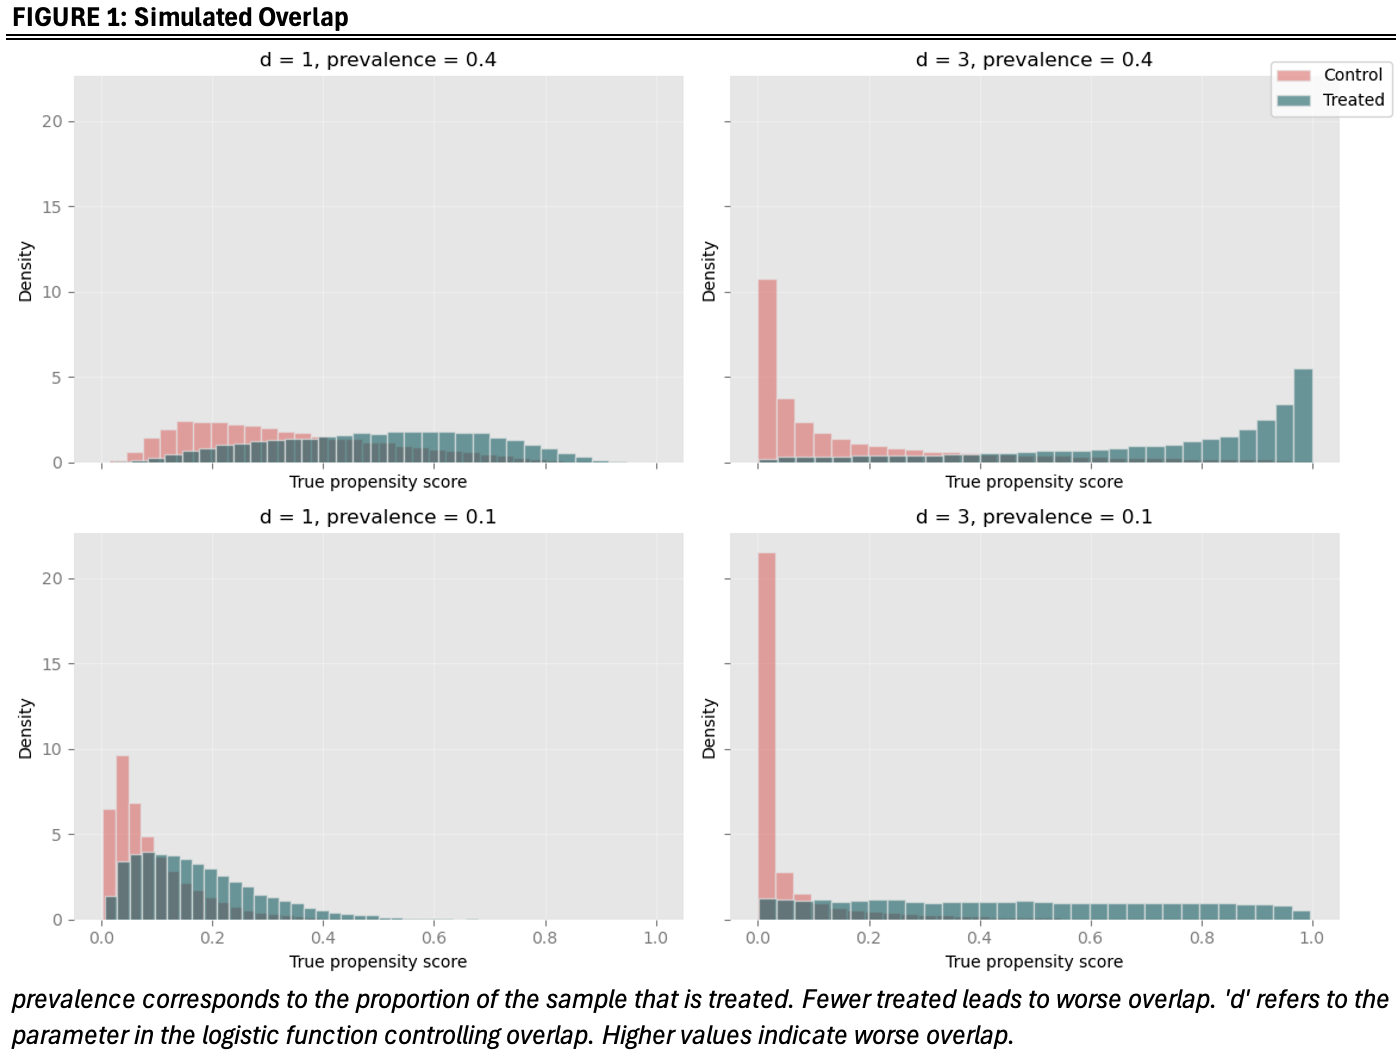
\includegraphics[width=1\textwidth]{Figure1}
\end{figure}

The top panels show scenarios when treatment prevalence is 40\%. The right side panels show when overlap is low. Accordingly, the top-left panel shows the best overlap scenario. On the other hand, the lower-right panel shows the worst overlap. That is, when treatment is rare and propensity scores are skewed toward zero for the control group only.

The untreated potential outcomes are given by a linear function of the following form:

$$
Y_i(0)
=
-0.5X_{i1}-0.8X_{i2}-1.2X_{i3}+0.8X_{i4}+0.8X_{i5}+1.0X_{i6}+\varepsilon_i,
\qquad
\varepsilon_i \sim \mathcal{N}(0,1).
$$

Finally the true treatment effect is modelled as heterogeneous, depending only on $X_{1}$ for simplicity. This is the key departure from the existing literature. I vary the parameter $h$ to simulate varying strength of heterogeneity.

$$
\tau(X_i)=1+hX_{i1}.
$$

The full observed outcome equation is then given by:

$$
Y_i = Y_i(0) + D_i\,\tau(X_i).
$$

\subsection{Model}

The model is a DR learner trained using the \textit{econML} package in Python. It is correctly specified given the data generating process, so that the propensity model is logistic and the outcome model is linear. The model is trained using 3-fold cross validation and the \textit{lbfgs} solver.

Given a heterogeneous treatment, the estimated model outcomes are CATEs. At each replication, the model predicts the CATE for every observation. The RMSE is computed as:

$$
\mathrm{RMSE}_{CATE}
=
\sqrt{
\frac{1}{n}\sum_{i=1}^{n}
\left(\hat{\tau}(X_i)-\tau(X_i)\right)^2
}.
$$

I take the average RMSE across all replications and call this metric (CATE RMSE). This captures the model’s error in estimating heterogeneous treatment effects.

The ATE can be computed by applying the Law of Iterated Expectations, and taking the mean over all CATEs for each replication. I compute the bias as the difference between the estimated and actual ATE. I take the mean over all replications and call this metric (ATE bias). This captures the size and direction of bias for the model’s average predictions.

Finally, I use ATE bias to compute the RMSE for ATE as:

$$
\hat{\tau}_{ATE}
=
\frac{1}{n}\sum_{i=1}^{n}\hat{\tau}(X_i).
$$

$$
\mathrm{RMSE}_{ATE}
=
\sqrt{
\frac{1}{R}\sum_{r=1}^{R}
\left(\hat{\tau}_{ATE}^{(r)}-\tau_S^{(r)}\right)^2
}.
$$

Where $r$ denotes the current replication. I call this metric the ATE RMSE.

I replicate each simulation 1000 times and report the main results using a sample size of 1000.

\section{Results}

\begin{table}[h!]
    \centering
    \footnotesize
    \resizebox{1.1\textwidth}{!}{
    \begin{threeparttable}
    \begin{tabular}{lccccccc}
        \multicolumn{8}{l}{\textbf{TABLE 1A: Monte Carlo Simulations for 40\% treatment prevalence}} \\
        \specialrule{0.08em}{0pt}{0pt}
        \specialrule{0.08em}{0.15em}{0.4em}
        \multicolumn{2}{l}{\textbf{}} & \multicolumn{3}{c}{High overlap (d=1)} & \multicolumn{3}{c}{Poor overlap (d=3)} \\
        \multicolumn{2}{l}{Heterogeneity} & \multicolumn{3}{c}{} & \multicolumn{3}{c}{} \\
        \multicolumn{2}{l}{Coefficient} & \textbf{ATE RMSE} & \textbf{ATE bias} & \textbf{CATE RMSE} & \textbf{ATE RMSE} & \textbf{ATE bias} & \textbf{CATE RMSE} \\
        \cmidrule(lr){3-5} \cmidrule(lr){6-8}
        \textbf{0}   & & 0.076885 & -0.000533 & 0.200646 & 0.396016 & -0.006599 & 0.585291 \\
        \textbf{0.5} & & 0.080147 & -0.001725 & 0.209276 & 0.545089 & -0.033129 & 0.703677 \\
        \textbf{1}   & & 0.085984 & -0.009473 & 0.230153 & 0.723276 & -0.089845 & 0.963303 \\
        \textbf{2}   & & 0.105725 & -0.018216 & 0.287694 & 1.157280 & -0.111568 & 1.422709 \\
        \bottomrule
    \end{tabular}
    \begin{tablenotes}
        \scriptsize
        \item \parbox{1.2\textwidth}{\textit{Results shown for sample of 1000. All else equal, greater heterogeneity in treatment effects results in greater RMSE. \\Error from heterogeneity is amplified when overlap is poor.}}
    \end{tablenotes}
    \end{threeparttable}}
\end{table}

\begin{table}[h!]
    \centering
    \footnotesize
    \resizebox{1.1\textwidth}{!}{
    \begin{threeparttable}
    \begin{tabular}{lccccccc}
        \multicolumn{8}{l}{\textbf{TABLE 1B: Monte Carlo Simulations for 10\% treatment prevalence}} \\
        \specialrule{0.08em}{0pt}{0pt}
        \specialrule{0.08em}{0.15em}{0.4em}
        \multicolumn{2}{l}{\textbf{}} & \multicolumn{3}{c}{High overlap (d=1)} & \multicolumn{3}{c}{Poor overlap (d=3)} \\
        \multicolumn{2}{l}{Heterogeneity} & \multicolumn{3}{c}{} & \multicolumn{3}{c}{} \\
        \multicolumn{2}{l}{Coefficient} & \textbf{ATE RMSE} & \textbf{ATE bias} & \textbf{CATE RMSE} & \textbf{ATE RMSE} & \textbf{ATE bias} & \textbf{CATE RMSE} \\
        \cmidrule(lr){3-5} \cmidrule(lr){6-8}
        \textbf{0}   & & 0.192684   & 0.000965   & 0.477177  & 43.034530   & 1.695425   & 10.722467 \\
        \textbf{0.5} & & 0.221392   & -0.051397  & 0.550236  & 54.653998   & -2.856936  & 15.561054 \\
        \textbf{1}   & & 0.360478   & -0.129710  & 0.821067  & 77.385386   & -2.529381  & 20.450878 \\
        \textbf{2}   & & 0.584636   & -0.253731  & 1.383130  & 198.672785  & -15.736825 & 43.754794 \\
        \bottomrule
    \end{tabular}
    \begin{tablenotes}
        \scriptsize
        \item \parbox{1.2\textwidth}{\textit{Results shown for sample of 1000. When treatment prevalence is low and overlap is poor, we essentially face a full violation \\of the overlap assumption. The model is completely unable to identify the CATEs.}}
    \end{tablenotes}
    \end{threeparttable}}
\end{table}

Table 1a shows results when treatment prevalence is 40\%. The first row shows a baseline model performance when no heterogeneity is present. These results have negligible difference those presented in (Yang et al., 2026) which reassures us that the data generating process and methodology are consistent with this paper.

As heterogeneity increases, we observe that the model errors also increase, all else being equal. Looking at the left-hand side of the table (when overlap is at its best) we see that the errors from increased heterogeneity remain small.

The right-hand side columns show the same models estimated when overlap is poor. Firstly, the top row shows that, when there is no heterogeneity, poor overlap alone causes higher model errors. Secondly, we observe that the errors arising from heterogeneity are amplified compared to the case with good overlap. Additionally, when heterogeneity is at its strongest, the CATE RMSE increases by almost 50\% relative to the next highest heterogeneity level. This suggests that greater heterogeneity paired with poor overlap can lead to substantial model errors, even when treatment prevalence is relatively balanced.

Table 1b shows the results when treatment prevalence is rare, leading to worse overlap. The left-hand side columns show us similar results. When overlap is poor, the model errors arising from greater heterogeneity are amplified. Greater heterogeneity leads to higher RMSE for both the CATE and ATE.

The right-hand columns show the worst overlap scenario, where control units all have propensities near zero, and only the treated have higher propensities. In this case, the model is shown to be practically useless, even when no heterogeneity is present. Overlap is so poor, and the propensities are so skewed that the model fails to identify the ATE or CATE at all. The model’s errors explode as we add increasing degrees of heterogeneity to the true treatment effects.

Figures 2 and 3 show how model performance varies as sample size varies.

\begin{figure}[ht]
	\centering
	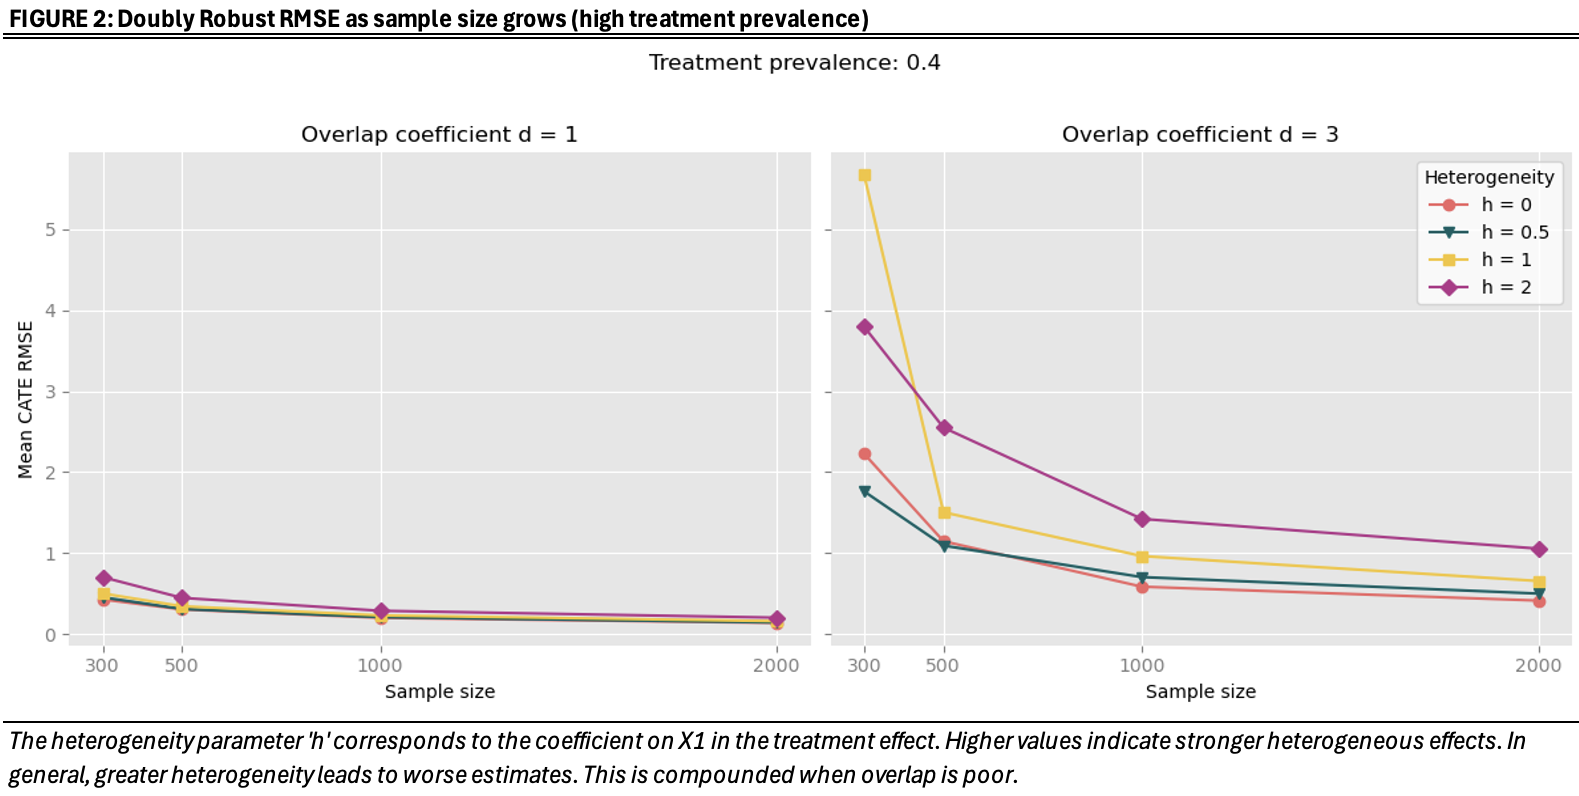
\includegraphics[width=1\textwidth]{Figure2}
\end{figure}

\begin{figure}[ht]
	\centering
	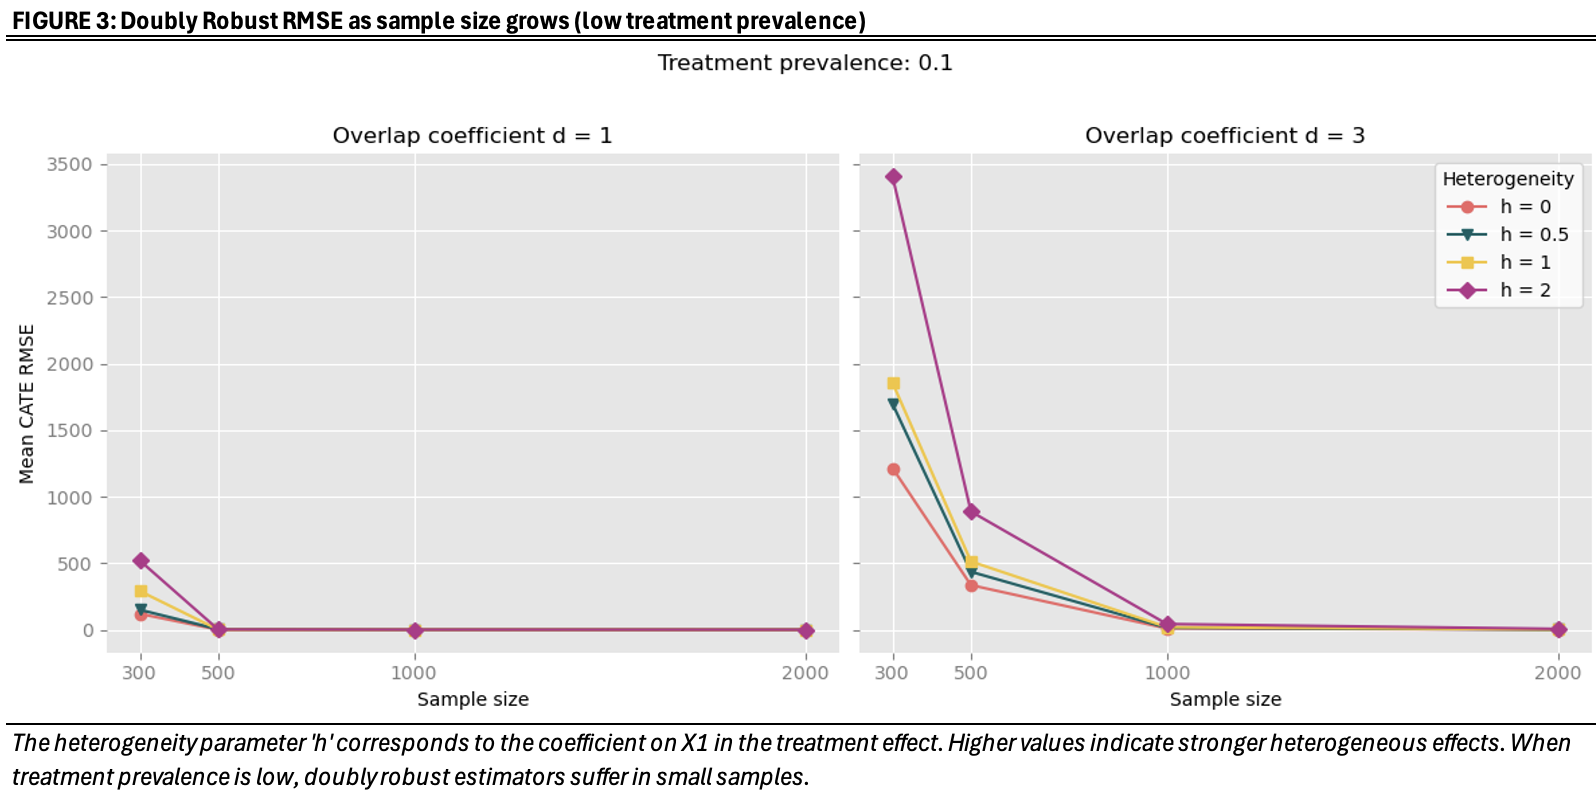
\includegraphics[width=1\textwidth]{Figure3}
\end{figure}

Figure 2 shows that, in general, greater heterogeneity leads to greater model errors. These errors are particularly pronounced in small samples, as there is not enough variation in the sample to identify causal effects. If we suspect strong heterogeneity in treatment effects, obtaining larger samples is of particular importance.

On the other hand, when overlap is very good the DR estimator is shown to achieve a low RMSE in small samples even when heterogeneity is present. This suggests that heterogeneity is not an issue when overlap between subjects is clearly satisfied. We may be content with a smaller sample if we can show clear overlap.

Figure 3 shows the case when treatment prevalence is rare. Note that this is on a different scale due to the fact that model RMSE explodes in very small sample sizes. In general, when overlap is poor and treatment is rare, the sample size must be high enough such that the treated population has enough variation for the causal effect to be estimated. In small samples, a 10\% prevalence makes up a very small number of observations (30-50 treated). Additionally, the model error arising from heterogeneity is shown to be much higher when sample size is small.

\section{Discussion}

Overall, the simulation results agree with the hypothesis that errors arising from heterogeneity are amplified by the DR estimator, causing large model errors when overlap is poor. In particular, stronger heterogeneity leads to greater model errors, which are amplified when overlap is poor. This motivates additional caution when estimating heterogeneous treatment effects with the DR estimator when the overlap assumption is uncertain.

Additionally, I found that the errors from heterogeneity are greater in smaller samples. This agrees with the intuition that a smaller population provides less variation to identify individual treatment effects. However, I found that this is not such an issue when the overlap assumption is comfortably satisfied. In the best overlap scenario, I showed that the CATE RMSE remains low even when there are strongly heterogeneous effects. This highlights that the only case when we may be satisfied with a small sample is when SUTVA and unconfoundedness are satisfied, and there is substantial overlap between groups. As overlap worsens, so does finite-sample performance.

Finally, I found that the overlap scenario where propensities are concentrated near zero is particularly fatal to the DR estimator. Regardless of the degree of heterogeneity, the DR model was unable to identify the causal effect when treatment prevalence was low and propensities were skewed. This again agrees with the hypothesis that the DR model amplifies errors from the outcome and propensity models, and that these errors are pronounced when propensities take on extreme values.

In light of these findings, it is clear that one should take caution with DR estimators when it is suspected that overlap is poor and heterogeneity is present. The DR estimator on its own is not equipped to deal with this issue. (Yang et al., 2026) suggest that the best way to deal with this issue is to shift the target population onto one where overlap is better. One method is by trimming the tails of the propensity distribution to remove the extreme propensity scores that are causing the largest model errors. This is shown to work, but it is undesirable in small samples as it entails removing a portion of the data.

(Li et al., 2019) discusses overlap weights as a potential remedy to poor overlap for the inverse probability weights estimator. This entails weighting each observation by down-weighting observations in the tails and up-weighting observations with high overlap. This reduces model error from poor overlap without removing observations.

Further research could investigate how effective these methods are when applied to the DR estimator with heterogeneous treatment effects, and how this varies for samples of different sizes.

In conclusion, I have shown that heterogeneous effects cause greater model errors for the DR estimator in finite samples, and that this error is amplified when overlap is poor. The errors from heterogeneity and poor overlap are particularly pronounced in small samples, and when treatment is rare. This motivates greater caution to be taken when using doubly robust methods to estimate causal effects in finite samples where there is significant heterogeneity and poor overlap.



\end{document}